\documentclass[border=3pt]{standalone}
% Preâmbulo compartilhado pelos diagramas TikZ da aula 13 (SLAM com EKF)
\usepackage[T1]{fontenc}
\usepackage[utf8]{inputenc}
\usepackage{lmodern}
\usepackage{amsmath}
\usepackage{xcolor}
\usepackage{tikz}
\usetikzlibrary{arrows.meta,angles,quotes,decorations.pathmorphing,decorations.pathreplacing,calc,
                positioning,shapes.geometric,shapes.misc,backgrounds,fit,
                math}

% Paleta (mesma dos SVGs originais)
\definecolor{dblue}{HTML}{2A5B8C}
\definecolor{dorange}{HTML}{B3541E}
\definecolor{dgreen}{HTML}{4A7C59}
\definecolor{dred}{HTML}{9C4B4B}
\definecolor{dcream}{HTML}{F4F1EA}
\definecolor{dshade}{HTML}{DDD7C9}

% Função gaussiana (não normalizada por padrão de escala visual)
\pgfmathdeclarefunction{gauss}{3}{%
  \pgfmathparse{1/(#3*sqrt(2*pi))*exp(-((#1-#2)^2)/(2*#3^2))}%
}

% Estilos comuns (prefixo d... para não colidir com chaves internas do pgf)
\tikzset{
  >={Stealth[length=2mm]},
  dguide/.style={gray!55, dashed, line width=0.4pt},
  daxis/.style={gray!60, line width=0.7pt, ->},
  dbody/.style={fill=black!3, draw=black!80, line width=1pt},
  dacc/.style={draw=dblue, line width=1pt},
  dlbl/.style={black!55, font=\small},
  dsub/.style={black!45, font=\footnotesize},
  dstate/.style={circle, draw=black!80, fill=dcream, line width=1pt,
                 minimum size=17mm, font=\large, inner sep=1pt},
  dobs/.style={circle, draw=black!80, fill=dshade, line width=1pt,
               minimum size=14mm, font=\large, inner sep=1pt},
  dbox/.style={rounded corners=2pt, draw=black!80, fill=dcream, line width=1pt,
               align=center, inner sep=6pt},
  dop/.style={circle, draw=black!80, fill=white, line width=1pt,
              minimum size=6mm, inner sep=0pt, font=\small},
  dtrans/.style={->, dblue, line width=1pt},
  dmeas/.style={->, dorange, line width=1pt},
  dcurve/.style={line width=1pt, dblue},
  dcurveb/.style={line width=1.4pt, dorange},
}

\begin{document}
\hyphenpenalty=10000 \exhyphenpenalty=10000 \tolerance=9999 \emergencystretch=3em
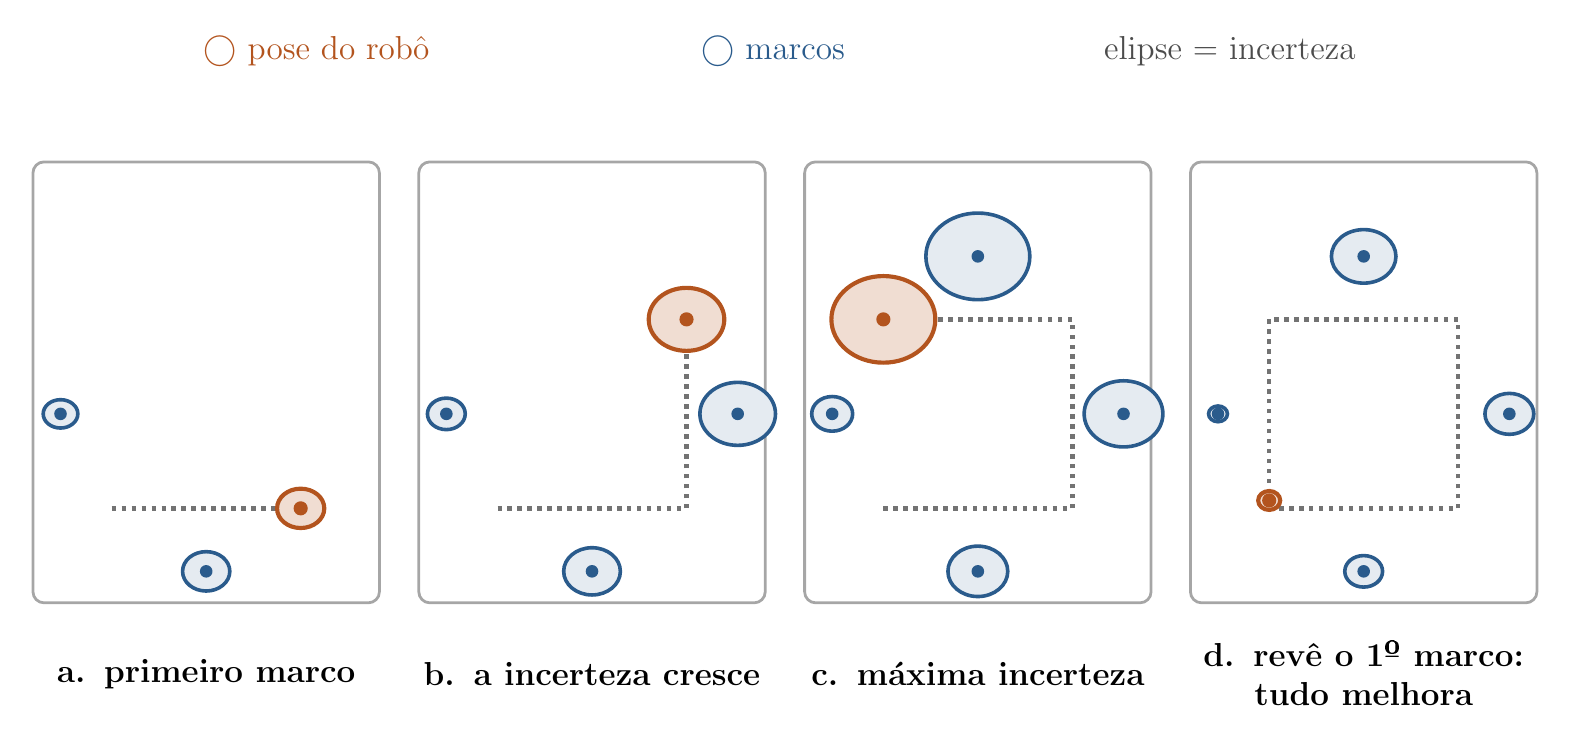
\begin{tikzpicture}[x=1cm,y=1cm]
\draw[black!35, line width=1pt, rounded corners=4pt] (0.0,0) rectangle (4.4,5.6);
\draw[black!55, dotted, line width=1.6pt] (1.0,1.2) -- (3.4,1.2);
\draw[dblue, fill=dblue!12, line width=1.3pt] (0.35,2.4) ellipse (0.22 and 0.18);
\fill[dblue] (0.35,2.4) circle (0.08);
\draw[dblue, fill=dblue!12, line width=1.3pt] (2.2,0.4) ellipse (0.3 and 0.25);
\fill[dblue] (2.2,0.4) circle (0.08);
\draw[dorange, fill=dorange!20, line width=1.5pt] (3.4,1.2) ellipse (0.3 and 0.25);
\fill[dorange] (3.4,1.2) circle (0.09);
\node[font=\large\bfseries, text width=4.3cm, align=center] at (2.2,-0.9) {a. primeiro marco};
\draw[black!35, line width=1pt, rounded corners=4pt] (4.9,0) rectangle (9.3,5.6);
\draw[black!55, dotted, line width=1.6pt] (5.9,1.2) -- (8.3,1.2);
\draw[black!55, dotted, line width=1.6pt] (8.3,1.2) -- (8.3,3.6);
\draw[dblue, fill=dblue!12, line width=1.3pt] (5.25,2.4) ellipse (0.24 and 0.2);
\fill[dblue] (5.25,2.4) circle (0.08);
\draw[dblue, fill=dblue!12, line width=1.3pt] (7.1000000000000005,0.4) ellipse (0.36 and 0.3);
\fill[dblue] (7.1000000000000005,0.4) circle (0.08);
\draw[dblue, fill=dblue!12, line width=1.3pt] (8.95,2.4) ellipse (0.48 and 0.4);
\fill[dblue] (8.95,2.4) circle (0.08);
\draw[dorange, fill=dorange!20, line width=1.5pt] (8.3,3.6) ellipse (0.48 and 0.4);
\fill[dorange] (8.3,3.6) circle (0.09);
\node[font=\large\bfseries, text width=4.3cm, align=center] at (7.1000000000000005,-0.9) {b. a incerteza cresce};
\draw[black!35, line width=1pt, rounded corners=4pt] (9.8,0) rectangle (14.200000000000001,5.6);
\draw[black!55, dotted, line width=1.6pt] (10.8,1.2) -- (13.200000000000001,1.2);
\draw[black!55, dotted, line width=1.6pt] (13.200000000000001,1.2) -- (13.200000000000001,3.6);
\draw[black!55, dotted, line width=1.6pt] (13.200000000000001,3.6) -- (10.8,3.6);
\draw[dblue, fill=dblue!12, line width=1.3pt] (10.15,2.4) ellipse (0.26 and 0.22);
\fill[dblue] (10.15,2.4) circle (0.08);
\draw[dblue, fill=dblue!12, line width=1.3pt] (12.0,0.4) ellipse (0.38 and 0.32);
\fill[dblue] (12.0,0.4) circle (0.08);
\draw[dblue, fill=dblue!12, line width=1.3pt] (13.850000000000001,2.4) ellipse (0.5 and 0.42);
\fill[dblue] (13.850000000000001,2.4) circle (0.08);
\draw[dblue, fill=dblue!12, line width=1.3pt] (12.0,4.4) ellipse (0.66 and 0.55);
\fill[dblue] (12.0,4.4) circle (0.08);
\draw[dorange, fill=dorange!20, line width=1.5pt] (10.8,3.6) ellipse (0.66 and 0.55);
\fill[dorange] (10.8,3.6) circle (0.09);
\node[font=\large\bfseries, text width=4.3cm, align=center] at (12.0,-0.9) {c. máxima incerteza};
\draw[black!35, line width=1pt, rounded corners=4pt] (14.7,0) rectangle (19.1,5.6);
\draw[black!55, dotted, line width=1.6pt] (15.7,1.2) -- (18.099999999999998,1.2);
\draw[black!55, dotted, line width=1.6pt] (18.099999999999998,1.2) -- (18.099999999999998,3.6);
\draw[black!55, dotted, line width=1.6pt] (18.099999999999998,3.6) -- (15.7,3.6);
\draw[black!55, dotted, line width=1.6pt] (15.7,3.6) -- (15.7,1.3);
\draw[dblue, fill=dblue!12, line width=1.3pt] (15.049999999999999,2.4) ellipse (0.12 and 0.1);
\fill[dblue] (15.049999999999999,2.4) circle (0.08);
\draw[dblue, fill=dblue!12, line width=1.3pt] (16.9,0.4) ellipse (0.24 and 0.2);
\fill[dblue] (16.9,0.4) circle (0.08);
\draw[dblue, fill=dblue!12, line width=1.3pt] (18.75,2.4) ellipse (0.31 and 0.26);
\fill[dblue] (18.75,2.4) circle (0.08);
\draw[dblue, fill=dblue!12, line width=1.3pt] (16.9,4.4) ellipse (0.41 and 0.34);
\fill[dblue] (16.9,4.4) circle (0.08);
\draw[dorange, fill=dorange!20, line width=1.5pt] (15.7,1.3) ellipse (0.14 and 0.12);
\fill[dorange] (15.7,1.3) circle (0.09);
\node[font=\large\bfseries, text width=4.3cm, align=center] at (16.9,-0.9) {d. revê o 1º marco: \textbf{tudo melhora}};
\node[font=\large, dorange] at (3.6,7.0) {$\bigcirc$ pose do robô};
\node[font=\large, dblue] at (9.4,7.0) {$\bigcirc$ marcos};
\node[font=\large, black!70] at (15.2,7.0) {elipse = incerteza};
\end{tikzpicture}
\end{document}
